% ===========================================================================
% Title:
% ---------------------------------------------------------------------------
% to create Type I fonts type "dvips -P cmz -t letter <filename>"
% ===========================================================================
\documentclass[11pt]{article}       %--- LATEX 2e base
\usepackage{latexsym}               %--- LATEX 2e base
%---------------- Wide format -----------------------------------------------
\textwidth=6in \textheight=9in \oddsidemargin=0.25in
\evensidemargin=0.25in \topmargin=-0.5in
%--------------- Def., Theorem, Proof, etc. ---------------------------------
\newtheorem{definition}{Definition}
\newtheorem{theorem}{Theorem}
\newtheorem{lemma}{Lemma}
\newtheorem{property}{Property}
\newtheorem{observation}{Observation}
\newtheorem{fact}{Fact}
\newenvironment{proof}           {\noindent{\bf Proof.} }%
                                 {\null\hfill$\Box$\par\medskip}
%--------------- Algorithm --------------------------------------------------
\newtheorem{algX}{Algorithm}
\newenvironment{algorithm}       {\begin{algX}\begin{em}}%
                                 {\par\noindent --- End of Algorithm ---
                                 \end{em}\end{algX}}
\newcommand{\step}[2]            {\begin{list}{}
                                  {  \setlength{\topsep}{0cm}
                                     \setlength{\partopsep}{0cm}
                                     \setlength{\leftmargin}{0.8cm}
                                     \setlength{\labelwidth}{0.7cm}
                                     \setlength{\labelsep}{0.1cm}    }
                                  \item[#1]#2    \end{list}}
                                 % usage: \begin{algorithm} \label{xyz}
                                 %        ... \step{(1)}{...} ...
                                 %        \end{algorithm}
%--------------- Figures ----------------------------------------------------
\usepackage{graphicx}
\usepackage{float}
\usepackage{graphicx}
\usepackage{caption}
\usepackage{subcaption}

\newcommand{\includeFig}[3]      {\begin{figure}[htb] \begin{center}
                                 \includegraphics
                                 [width=4in,keepaspectratio] %comment this line to disable scaling
                                 {#2}\caption{\label{#1}#3} \end{center} \end{figure}}
                                 % usage: \includeFig{label}{file}{caption}


% ===========================================================================
\begin{document}
% ===========================================================================

% ############################################################################
% Title
% ############################################################################

\title{An Effective way to optimize performance and battery life of smart devices using multi-kernel approach}


% ############################################################################
% Author(s) (no blank lines !)
\author{
% ############################################################################
Sadid Rafsun Tulon\\
School of Computer Science\\
University of Ottawa\\
Ottawa, Canada\\
{\em stulo080@uottawa.ca}
% ############################################################################
} % end-authors
% ############################################################################

\maketitle

% ############################################################################
% Abstract
% ############################################################################
\begin{abstract}
Improving the performance and battery life of smart devices is modern technology's most vital goal. As lowing transistor size becomes increasingly complex and battery technology has plateaued, other methods to increase performance and decrease power consumption are being explored relentlessly. While there are many techniques available, this paper addresses how to improve the performance and battery life of modern battery-powered smart devices using a new multi-kernel system technique. The main goal of this paper is to examine the potential of multi-kernel systems and compare them against Linux systems.
\end{abstract}

% ############################################################################
\section{Introduction} \label{intro}
% ############################################################################

Smart devices have become an integral part of our life. Many of the smart devices are battery-powered. The current battery technology is the most significant handicap of portable smart devices right now. As CPUs and systems on a chip(SoC) improve their efficiency, things are getting better. However, modern software also demands more processing power, which faster drains the battery. The lightweight kernels can extend battery life much further, but their software compatibility is far from ideal. Now that battery technology has reached a plateau and transistors in the semiconductors are also close to reaching their size limit, we are in need of an alternate way of achieving better battery life without compromising performance and compatibility. A new approach using multiple operating system (OS) kernels can help mitigate this problem. Almost all modern chips are multi-core. We can use these multi-core chips to run multiple OS kernels at the same time. Ideally, one of the kernels is a lightweight kernel for better performance and battery life and a monolithic kernel for better compatibility. The system can switch between the kernels, run them simultaneously, or stop them from running depending on the need. This way, we will be able to get better battery life while still retaining the software compatibility. This research is an effort to optimize performance, compatibility, and battery life by utilizing a multi-kernel approach while using existing battery technology. 

In this project, the idea is to research if we fit two operating systems for both cores of multi-core processors individually and how they perform.

% ############################################################################
\section{Literature Review} \label{litrev}
% ############################################################################

\subsection{Different types of kernels}
The current hardware technology is changing rapidly. The software is struggling to keep up with this rapid change. Thus it has become very challenging to optimize software for a specific hardware\cite{DEL02}. So we need a new OS structure that can be as scalable as needed. This is where LWKs and unikernels come in handy. Multi-core processors are used in the majority of current systems. We can leverage this to our advantage.\\

Light Weight Kernels (LWKs) are not a new concept. They have been here for at least 30 years \cite{DEL04}. However, they are only gaining popularity in these past couple of years because of High-Performance Computing (HPC). HPC necessitates tremendous scalability, which the Full-Weight Kernel (FWKs) take a long time to adjust to. LWKs work exceptionally well with highly scalable systems as they have a simple codebase.Table \ref{table:1} describes the Design goals of LWKs and FWKs\\


\begin{table}
\begin{tabular}{ c c c }
\hline
 Design goal & LWK & FWK \\ [0.5ex] 
\hline
 Target & massively parallel systems & laptops, desktops, servers \\ 
 Support & scalable applications & everything under the sun \\  
 Dev. environment for & parallel applications & business, games, commerce, etc. \\
 Emphasis & effciency & functionality  \\ 
 Resources & maximize use & fair sharing, QoS  \\
 Time to completion & minimal & when needed  \\
\end{tabular}
\caption{Design goals of LWKs and FWKs \cite{DEL04}}
\label{table:1}
\end{table}

There is also a new type of single address space operating system called unikernels. They are minimalistic single-purpose operating systems made from library os [unikernel]. As they are very specialized, it is easy to optimize them for hardware. Like LWKs, unikernels are also very lightweight, sometimes unikernels are lighter than LWKs \cite{DEL13}. Moreover, like LWKs they are also extremely resource efficient \cite{DEL16}.

Figure~\ref{fig1} shows application stack on monolithic OS vs Unikernel.

\includeFig{fig1}{Figures/figure.png}{Application stack on monolithic OS vs Unikernel \cite{DEL11}}



In this paper, we will be treating both unikernal and LWK as the sub kernel as they both have better performance and efficiency than FWKs and have limited compatibility with the standard  APIs \cite{DEL03}, \cite{DEL01}. Another major issue of LWKs and unikernels are driver support. As they have a simple codebase mainly focusing on performance, they are missing many advanced features that FWKs have \cite{DEL03} \cite{DEL14}.


\subsection{Multi-Kernel systems}
Multi-kernel operating systems have been presented as a way to improve system performance and efficiency without sacrificing software and hardware compatibility. Multikernel OS runs both FWK and sub kernel side by side divides their tasks \cite{DEL01}. The sub kernel is usually responsible for the high-performance tasks, and FWK is there for ensuring compatibility, driver support and serves as a backup system \cite{DEL03}. In high-performance supercomputers, this system performs admirably. 

Figure~\ref{fig2} shows the system architecture of a multikernel system.

\includeFig{fig2}{Figures/figure2.png}{System Architectural Overview of Multi-kernel \cite{DEL04}}

This paper will explore if we can use this multi-kernel method on battery-powered smart devices. We will compare performance and power efficiency between a single Linux kernel system and a multi-kernel system. As batteries have a very small capacity, ensuring longer battery life while maintaining consistent performance is crucial for this project. Thus performance and power efficiency will be the main focuses of this research project.

% ############################################################################
\section{Problem Statement} \label{problemStatement}
% ############################################################################

Moore’s Law \cite{DEL15} is reaching a physical limitation. Industry still trying to come up with clever methods to to shrink it even further but those methods are really expensive and complex. Battery technology has also slowed down. But demand for battery powered devices are increasing exponentially. So enhancing performance and battery life takes top priority. As we are close to technical limitation of hardware, we need a approach to improve performance and battery life that is not constrained by hardware. 

% ############################################################################
\section{Proposed Solution} \label{proposedSolution}
% ############################################################################

Most of our modern chips are using multiple cores. Multi-kernel system is a new promising method that can leverage these multi-core chips. As mentioned before multikernel system is a method of running two kernel simultaneously on a device.One main advantage of this system is, it has a potential to improve existing devices using software update, not only the new devices. We will evaluate if multikernel systems has potential to solve performance and battery life problem. 


% usage: \includeFig{label}{file}{caption}

% ############################################################################
\section{Experiments and Evaluation} \label{expEval}
% ############################################################################

\includeFig{fig4}{Figures/unikraftboot.png}{Bootscreen of Unikraft running Flask server}
\includeFig{fig5}{Figures/wolinux.jpg}{Unikraft Flask server vs Linux native Flask server (without OS) power consumption}

\includeFig{fig6}{Figures/wlinux.jpg}{Unikraft Flask server vs Linux native Flask server (with OS) power consumption}


\begin{figure}
\centering
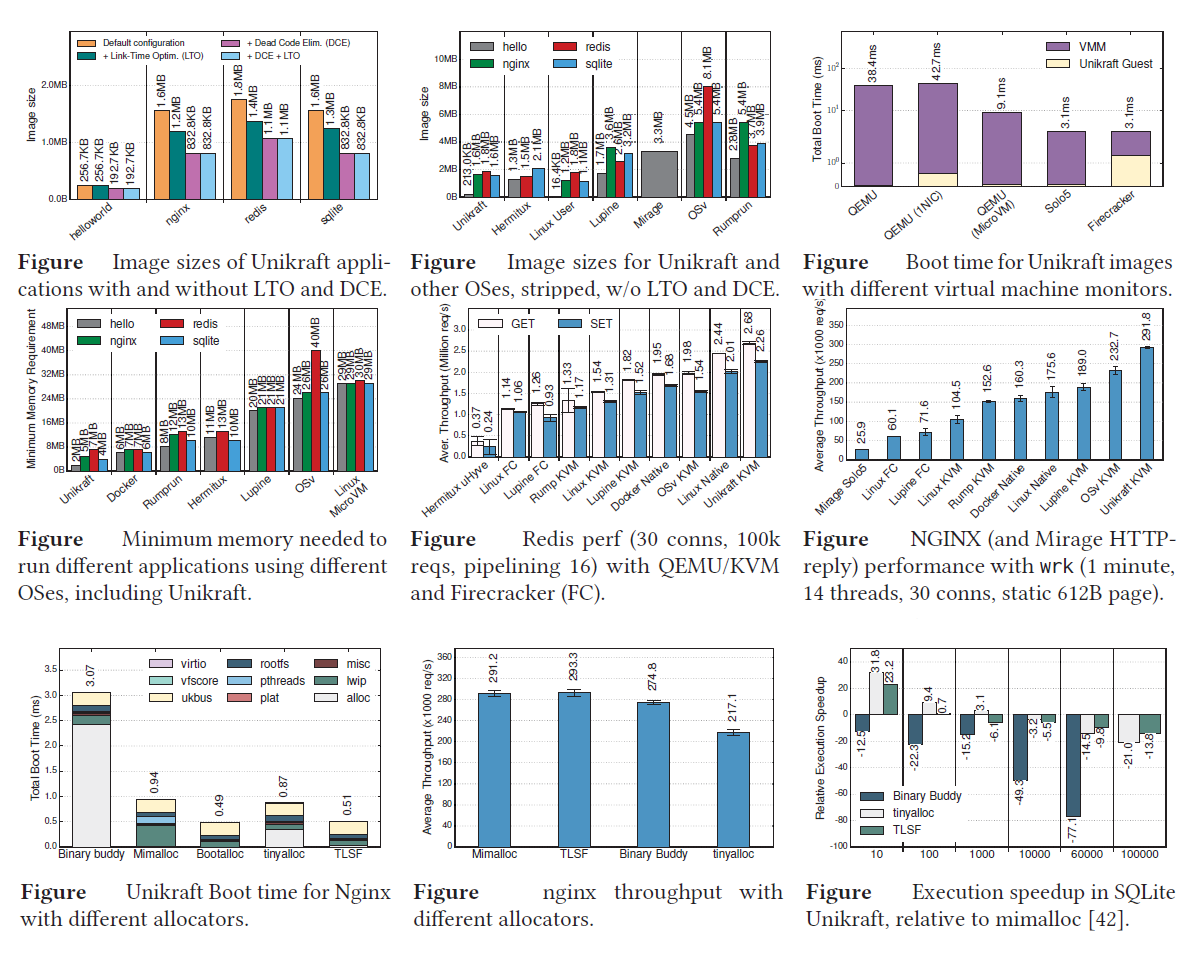
\includegraphics[width=.85\textwidth]{Figures/12.png}
\caption{Performance overview of Unikraft and comparison against competitors\cite{DEL14}}
\label{fig:6}
\end{figure}



The following experiments are done with a machine using Intel core I5 4500H 4 core CPU  clocked at 2.50 GHz, 8 gigabytes of ram. Primary operating systems were Ubuntu and CentOs depending on the situation. We tried to compile and test various open-source LWKs and Unikernels such as Azalea, HermitCore, mckernel, MirageOs, Unikraft. 
Table \ref{table:2}  describes the summery of each experiment.



\begin{table}[htbp]
\resizebox{\columnwidth}{!}{
\begin{tabular}{ccccc}
\hline
 Kernel&Main Linux OS&Architecture&Status&Result \\ 
\hline
 Azalea & CentOs & x86 & Failed to install & Fail\\
 
 Hermitcore & Ubuntu & x86 & Failed to compile on machine  & Fail \\ 
 mckernel & CentOs & x86 & Failed to compile on machine & Fail \\ 
 mckernel & CentOs & arm64 & Failed to compile on machine & Fail \\ 
 MirageOs & Ubuntu & x86 & Successfully compiled on machine  & Partial Success \\ 
  &  & & but failed to boot anything other  &  \\ 
  &  & &  than helloworld &  \\ 
 MirageOs & RaspbianOS & arm64 & Failed to compile on machine & Fail \\ 
 Unikraft & Ubuntu & x86 & Successfully compiled and ran flask & Success\\
  &  & & server  &  \\ 
 Unikraft & RaspbianOS & arm64 & Successfully compiled on machine  & Partial Success \\ 
  &  & & but failed to boot anything other  &  \\ 
  &  & &  than helloworld &  \\ 
 
 
\hline
\end{tabular}}
\caption{Experiment with various kernels}
\label{table:2}
\end{table}


From Table \ref{table:2}, we can see that only Unikraft fully worked on our system. The rest of the kernels refused to compile or run. 

We also tried to compile and test the kernels mentioned above on the Raspberry pi 4 4 gigabyte model. Only helloworld module of Unikraft ran properly.  


We suspect such a situation occurred because these kernels are built for server CPUs such as Intel Xeon and Fujitsu A64FX \cite{DEL01} \cite{DEL02} \cite{DEL04}. Almost all of the LWKs and unikernels and specialized for servers, so it is understandable that consumer-grade CPUs are incompatible with them. So in the end, we were not able to fully implement multikernel system. While we were able to boot unikraft it was not true multikernel system as unikraft was running on kvm.


As only Unikrft ran properly on our main system, we will mainly focus on Unikraft. We have been able to run flask server on Unikraft. While testing, the boot time of unikraft was found 3 seconds on average. Unikraft flask server consumes 60 milliwatt on average. On the other hand native linux flask server process consumes 20 milliwatt on average. But if we also include Linux power consumption, total power consumption will be 8000 milliwatt on average on freshly booted system.

Figure~\ref{fig4} is the bootscreen of Unikraft running Flask server.

Figure~\ref{fig5} is comparison of power consumption between Unikraft Flask server and Linux native Flask server without including whole Linux power consumption. 


Figure~\ref{fig6} is comparison of power consumption between Unikraft Flask server and Linux native Flask server without including whole Linux power consumption.


Unfortunately, due to lack of proper hardware, we were unable to verify the full potential of of multikernel system. But this system still shows potential. Our experiment shows that this system uses less power if implemented properly. We have also seen from earlier research that this system also performs better in most cases \cite{DEL14}. 



% ############################################################################
\section{Conclusions} \label{concl}
% ############################################################################


\subsection{Conclusions} 
In conclusion, multikernel system is a promising concept but needs more support. Currently, some kernels such as Unikraft, Include os, mirage os are receiving decent support but there are still room for improvement. As the support for these kernels gets better, they should also be more available to wider range of systems.
\subsection{Summary of Contributions}
In this paper, we tried to explore if the multikernel system is viable alternative method to improve performance and battery life. We tried to test several mainstream sub kernels on consumer level hardware such as generic laptop and raspberry pi. We also measured boot time and power consumption on Unikraft. But we could not boot anything meaningful on raspberry pi. As our main target system for the project is battery powered devices, arm powered raspberry pi should have been the main target system. Unfortunately, due to lack of support, raspberry pi was not able to boot anything that can be measured properly.
\subsection{Future Work}
Future work includes making multikernel system more available. To do that we need to make existing kernels work with more devices or create a new configurable kernel from ground up with large array of hardware support in mind.


% ############################################################################
% Bibliography
% ############################################################################
\bibliographystyle{plain}
\bibliography{my-bibliography}     %loads my-bibliography.bib

% ============================================================================
\end{document}
% ============================================================================
